\subsection{An\'alisis temporal}

Aparte de analizar convergencia y precisi\'on, decidimos realizar un experimento para poder observar los tiempos de ejecuci\'on de los m\'etodos implementados. El experimento consiste en observar la relaci\'on entre precisi\'on del resultado obtenido contra la cantidad de ciclos de reloj insumidos por el m\'etodo. Por este motivo, el \'unico par\'ametro variable fue la precis\'on, dejando $\alpha$ , y valores iniciales fijos para todos los m\'etodos. La h\'ipotesis que manejamos es que a mayor precisi\'on el m\'etodo tiene que ejecutarse m\'as iteraciones y por lo tanto el tiempo de ejecuci\'on aumenta. Para obtener los tiempos de ejecuci\'on de cada m\'etodo ejecutamos cada m\'etodo 1000 veces, en condiciones normales de uso de CPU, midiendo en cada iteraci\'on el tiempo insumido. Luego a este valor le calculamos el promedio. 

\begin{figure}[H]
	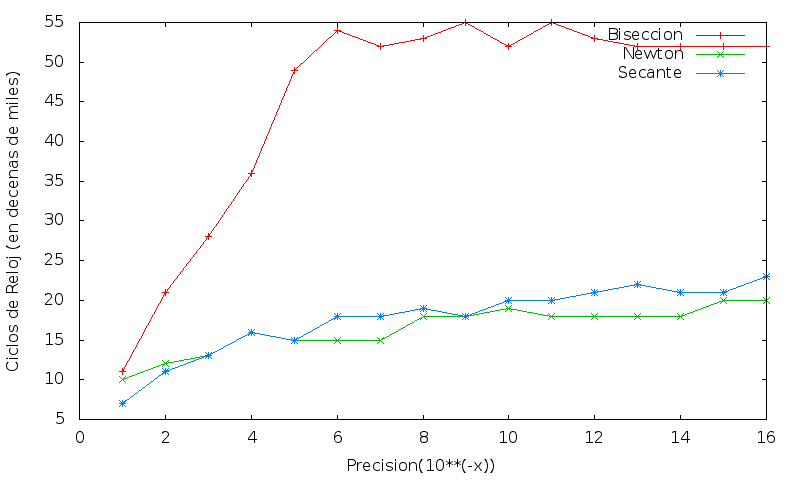
\includegraphics[scale = 0.5]{../Imagenes/tiempos/tiempos_precision_f.png}
	\caption{Gr\'afico de an\'alisis temporal para la funci\'on $f(x)$ con $\alpha = 0.25$.}
\end{figure}

\begin{figure}[H]
	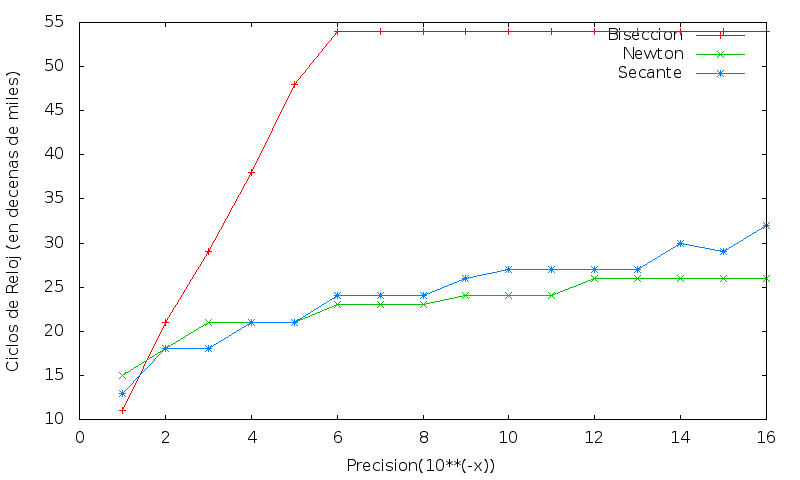
\includegraphics[scale = 0.5]{../Imagenes/tiempos/tiempos_precision_e.png}
	\caption{Gr\'afico de an\'alisis temporal para la funci\'on $e(x)$ con $\alpha = 0.5$.}
\end{figure}


En la figura 16 se representan los resultados obtenidos por el experimento para la funci\'on $f(x)$. Se puede observar que se cumple la hip\'otesis que a mayor precisi\'on, mayores son la cantidad de ciclos insumidos por el m\'etodo. Tambi\'en se puede ver el efecto del orden de convergencia cuadr\'atico de Newton, en comparaci\'on al lineal de Bisecci\'on y el supralineal de Secante, porque es el m\'etodo que m\'as r\'apido alcanza una soluci\'on y por lo tanto consume menos ciclos de reloj. Asimismo se observan los mismos resultados en la figura 17, la que result\'o del experimento con la funci\'on $e(x)$.


Para ambas figuras se puede observar que a partir de ciertas precisiones el m\'etodo tarda tiempos similares; esto se puede atribuir a dos factores: cantidad de iteraciones m\'aximas o aumento de precisi\'on entre iteraciones. La cantidad de iteraciones m\'aximas es un par\'ametro con el cual se decide hasta donde calcula el m\'etodo en caso de no cumplirse la condici\'on de parada; de esta manera si para cierta precisi\'on se alcanz\'o la cantidad de iteraciones m\'aximas entonces es natural asumir que para precisiones mayores siempre se va alcanzar ese punto, de forma que los m\'etodos van a tener un tiempo de ejecuci\'on bastante similar. El segundo factor, el de aumento de precisi\'on, depende de los m\'etodos. De una iteraci\'on a otra la soluci\'on obtenida se mejora en cierta precisi\'on. Si ese aumento es bastante mayor a la precisi\'on que se est\'a considerando entonces podr\'ia pasar que el aumento de precisi\'on del experimento sea menor a ese aumento entre iteraciones.
 
